\def\layersep{1cm}
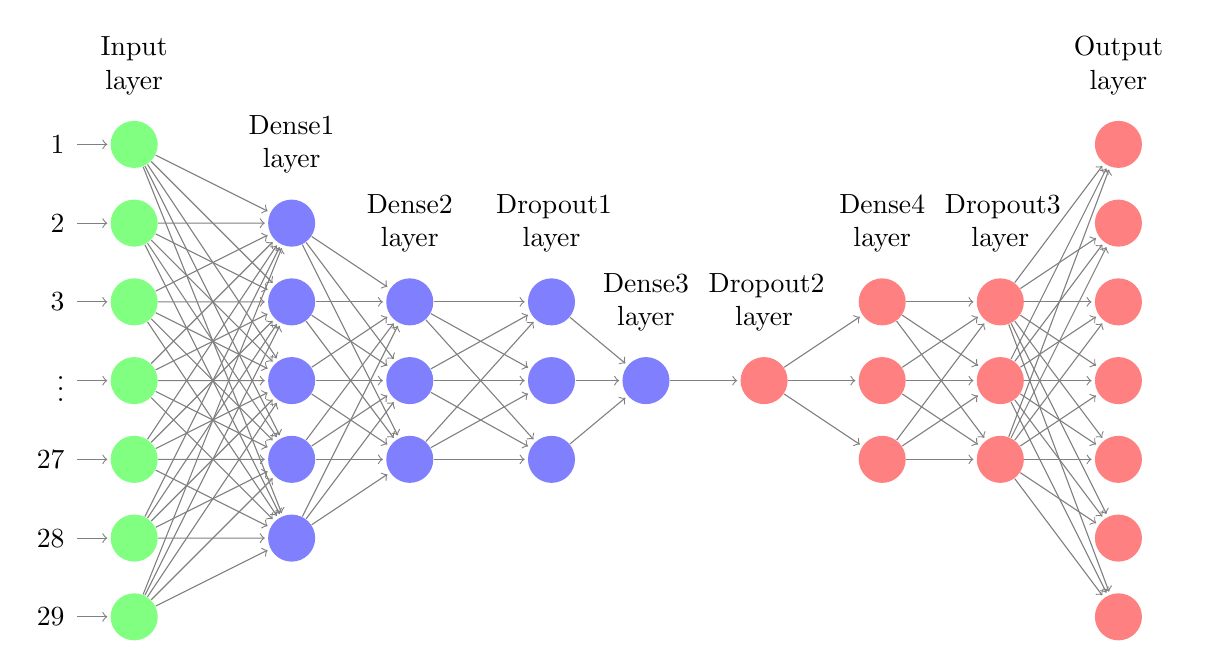
\begin{tikzpicture}[shorten >=1pt,->,draw=black!50, node distance=\layersep]
	\tikzstyle{every pin edge}=[<-,shorten <=1pt]
	\tikzstyle{neuron}=[circle,fill=black!25,minimum size=17pt,inner sep=0pt]
	\tikzstyle{input neuron}=[neuron, fill=green!50];
	\tikzstyle{decoder neuron}=[neuron, fill=red!50];
	\tikzstyle{encoder neuron}=[neuron, fill=blue!50];
	\tikzstyle{annot} = [text width=4em, text centered]
	
	% Draw the input layer nodes
	\foreach \y in {1,...,7}{
		% This is the same as writing \foreach \name / \y in {1/1,2/2,3/3,4/4}
		\ifnum\y<4
		\node[input neuron, pin=left: \y] (I-\y) at (0,-\y) {};
		\fi
		\ifnum\y=4
		\node[input neuron, pin=left: \vdots] (I-\y) at (0,-\y) {};
		\fi
		\ifnum\y=5
		\node[input neuron, pin=left: 27] (I-\y) at (0,-\y) {};
		\fi
		\ifnum\y=6
		\node[input neuron, pin=left: 28] (I-\y) at (0,-\y) {};
		\fi
		\ifnum\y=7
		\node[input neuron, pin=left: 29] (I-\y) at (0,-\y) {};
		\fi
	}
	
	% Draw the Dense_1 layer nodes
	\foreach \y in {2,3,4,5,6}{
		\node[encoder neuron, right of=I-4] (H1-\y) at (\layersep,-\y cm) {};
	}
	% Draw the Dense_2 layer nodes
	\foreach \y in {3,4,5}{
		\node[encoder neuron, right of=H1-3] (H2-\y) at (\layersep*2.5,-\y cm) {};
	}
	% Draw the Dropout_1 layer nodes
	\foreach \y in {3,4,5}{
		\node[encoder neuron, right of=H2-2] (H3-\y) at (\layersep*4.3,-\y cm) {};
	}
	% Draw the Dense_3 layer nodes
	\foreach \y in {4}
	\node[encoder neuron, right of=H3-2] (H4-\y) at (\layersep*5.5,-\y cm) {};
	
	% Draw the Dropout_2 layer nodes
	\foreach \y in {4}
	\node[decoder neuron, right of=H4-1] (H5-\y) at (\layersep*7,-\y cm) {};
	
	% Draw the Dense_4 layer nodes
	\foreach \y in {3,4,5}
	\node[decoder neuron, right of=H5-1] (H6-\y) at (\layersep*8.5,-\y cm) {};
	
	% Draw the Dropout_3 layer nodes
	\foreach \y in {3,4,5}
	\node[decoder neuron, right of=H6-2] (H7-\y) at (\layersep*10,-\y cm) {};
	
	% Draw the output layer node
	\foreach \y in {1,...,7}
	\node[decoder neuron, right of=H7-2] (H8-\y) at (\layersep*11.5,-\y cm){};
	
	% Connect every node in the input layer with every node in the
	% Dense_1 layer.
	\foreach \source in {1,...,7}
	\foreach \dest in {2,3,4,5,6}
	\path (I-\source) edge (H1-\dest);
	% Connect every node in the Dense_1 layer with every node in the
	% Dense_2 layer.
	\foreach \source in {2,3,4,5,6}
	\foreach \dest in {3,4,5}
	\path (H1-\source) edge (H2-\dest);
	% Connect every node in the Dense_2 layer with every node in the
	% Dropout_1 layer.
	\foreach \source in {3,4,5}
	\foreach \dest in {3,4,5}
	\path (H2-\source) edge (H3-\dest);
	% Connect every node in the Dropout_1 layer with every node in the
	% Dense_3 layer.
	\foreach \source in {3,4,5}
	\path (H3-\source) edge (H4-4);
	% Connect every node in the Dense_3 layer with every node in the
	% Dropout_2 layer.
	\path (H4-4) edge (H5-4);
	% Connect every node in the Dropout_2 layer with every node in the
	% Dense_4 layer.
	\foreach \dest in {3,4,5}
	\path (H5-4) edge (H6-\dest);
	% Connect every node in the Dense_4 layer with every node in the
	% Dropout_3 layer.
	\foreach \source in {3,4,5}
	\foreach \dest in {3,4,5}
	\path (H6-\source) edge (H7-\dest);
	% Connect every node in the Dropout_3 layer with every node in the
	% Dense_5 layer.
	\foreach \source in {3,4,5}
	\foreach \dest in {1,...,7}
	\path (H7-\source) edge (H8-\dest);
	
	% Annotate the layers
	\node[annot,above of=H1-2, node distance=1cm] {Dense1 layer};
	\node[annot,above of=H2-3, node distance=1cm] {Dense2 layer};
	\node[annot,above of=H3-3, node distance=1cm] {Dropout1 layer};
	\node[annot,above of=H4-4, node distance=1cm] {Dense3 layer};
	\node[annot,above of=H5-4, node distance=1cm] {Dropout2 layer};
	\node[annot,above of=H6-3, node distance=1cm] {Dense4 layer};
	\node[annot,above of=H7-3, node distance=1cm] {Dropout3 layer};
	\node[annot,above of=I-1] {Input layer};
	\node[annot,above of=H8-1] {Output layer};
	
\end{tikzpicture}